\chapter{Latent Variable Models}
\section{Introduction}
\subsection{Motivation of Latent Variable Models}
\label{sec:intro_motivation}
If we knew a corresponding latent variable for each observation, then modelling might be easier. Imagine, how can we find $z^* = \argmax_{z} p(\mathbf{x|z})$ for the data $\mathbf{x}$ as shown in Fig. \ref{fig:clusters}(b)

\begin{figure}[h]
	\begin{center}			
		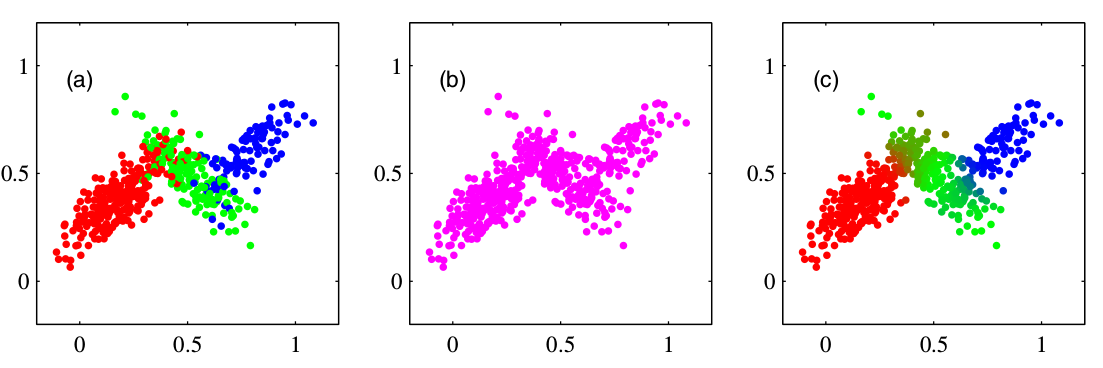
\includegraphics[scale=0.25]{./images/generative/latent.png}
	\end{center}
	\caption{(a) Complete data set $p(\mathbf{x|z})$. (b) Incomplete data set $p(\mathbf{x})$. (c) Inference result}
	\label{fig:clusters}
\end{figure}
For example, we want to model the complete data set $p(\mathbf{x|z})$ under the i.i.d. assumption 
\begin{equation*}
p(\mathbf{x}_i, \mathbf{z}_i|\boldsymbol{\theta}) = 
\begin{cases}
p(\mathcal{C}_1)p(\mathbf{x}_i|\mathcal{C}_1) \textrm{ if } z_i=0\\
p(\mathcal{C}_2)p(\mathbf{x}_i|\mathcal{C}_2) \textrm{ if } z_i=1\\
p(\mathcal{C}_3)p(\mathbf{x}_i|\mathcal{C}_3) \textrm{ if } z_i=2\\
\end{cases}
\end{equation*}
\begin{align*}
p(\mathbf{x}_1, \mathbf{x}_2,...,\mathbf{x}_N, \mathbf{z}_1, \mathbf{z}_2, ..., \mathbf{z}_N|\boldsymbol{\theta}) = \prod_{n=1}^{N}\prod_{k=1}^{K}\pi_k^{z_{nk}}\mathcal{N}(\mathbf{x}_n|\boldsymbol{\mu}_k, \boldsymbol{\Sigma}_k)^{z_{nk}}
\end{align*}
, where $\pi_k=p(\mathcal{C}_k)$ and $p(\mathbf{x}_i|\mathcal{C}_k)=\mathcal{N}(\mathbf{x}_n|\boldsymbol{\mu}_k, \boldsymbol{\Sigma}_k)$. However, in many cases, it is not observable. 

%In this case, what we can only do is find a posterior $p(\mathbf{x}|\mathbf{z},\boldsymbol{\theta})$.
